

When using Ellipsis, it should be clear what the pattern is

%-------------------------------------%


%-----------Reference to section 2.2.3 Power Sets




%-------------------------------------%

%----(Reference to Section 2.2.2 Cardinality)



%--------------------------------------%
\subsection*{ Three Sets }

%- Section 2.3.5 %- Associative Law %- Distribution Law





%-------------------------------------% %- Section 3
Propositional Logic A statement is a declarative sentence that
is either true or false.
\begin{itemize}
\item $\tilde q$ not q \item $p \vee q$ \item $p \wedge \tilde
q$
\end{itemize}

%%%%%%%%%%%%%%%%%%%%%%%%%%%%%%%%%%%%%%%%%%%

\item 
Let A, B be subsets of the universal set \mathcal{U}.

Use membership tables to prove De Morgan's Laws.

---------------------------------------------
Draw a venn diagram to show three subsets A,B and C of a universal set U intersecting in
the most general way?
How are sets $X$ and $Z$ related?
Can you describe each of the subsets X,Y and Z in terms  of the
sets A,B,C using the operations union intersection and set complement.

Construct Membership tables for each of the sets
(A-B) - C
A-(B- C)

(A-B) -C = A-(B-C)
A



\begin{itemize}
\item[a.] (1 mark) Write out the sample space for the outcomes for both players A and B.
\item[b.] (1 mark) Write out the sample space for the outcomes of C, where C is the difference of the two scores (i.e. B-A)
\item[c.] (1 mark) Are the sample points for the sample space of C equally probable? Provide a brief justification for your answer.
\end{itemize}

%----------------------------------------------------------%
\newpage
\section*{Section B: Set Operations}
\begin{itemize}
\item[B.1] complement of A $A^{\prime}$
\item[B.2] Union $A \cup B$
\item[B.3] Intersection $A \cap B$
\item[B.4] Relative Difference $A \otimes B$
\item[A.5]
\item[A.6]
\item[A.7]
\item[A.8]
\end{itemize}
\newpage


\subsection*{Operation on Sets}

\begin{itemize}
\item The complement of Set
\item Binary Operations
\begin{itemize}
\item Union
\item Intersection
\end{itemize}
\item Membership tables
\item Laws for Combining Sets
\end{itemize}
%----------------------------------------------------------%
\subsection*{Membership Tables}
Using membership tables
\begin{tabular}{|ccc|c|c|c|}
\hline
% after \\: \hline or \cline{col1-col2} \cline{col3-col4} ...
A & B & C & x & y & z \\\hline
0 & 0 & 0 & 1 & 1 & 1 \\
0 & 0 & 1 & 0 & 0 & 1 \\
0 & 1 & 0 & 0 & 0 & 1 \\
0 & 1 & 1 & 0 & 0 & 1 \\
1 & 0 & 0 & 1 & 0 & 1 \\
1 & 0 & 1 & 1 & 0 & 1 \\
1 & 1 & 0 & 0 & 0 & 1 \\
1 & 1 & 1 & 1 & 0 & 1 \\
\hline
\end{tabular}


\subsection*{Associative Laws}
\[ (A \cup B) \cup C =  A \cup (B \cup C)  \]
\[ (A \cap B) \cap C =  A \cap (B \cap C)  \]

\subsection*{Distributive Laws}
\[ (A \cup B) \cap C =  (A \cup B) \cap (A \cup C)  \]
\[ (A \cap B) \cup C =  (A \cap B) \cup (A \cap C)  \]


\[ (A \cup B) \cap B^{\prime} \]
%----------------------------------------------------------%

%----------------------------------------------------------%
\newpage



%-------------------------------------%
% Binary Operations on Sets (2.3.2)
% Union , Intersection, Symmetric Difference
% Set Difference



\subsection{Ellipsis}

When using Ellipsis, it should be clear what the pattern is

%-------------------------------------%


%--------------------------------------%
\subsection*{ Three Sets }

%- Section 2.3.5 %- Associative Law %- Distribution Law

%-------------------------------------% %- Section 3
Propositional Logic A statement is a declarative sentence that
is either true or false.
\begin{itemize}
\item $\tilde q$ not q \item $p \vee q$ \item $p \wedge \tilde
q$
\end{itemize}



%======================================================================================= %

Question 5


Let A, B be subsets of the universal set $\mathcal{U}$.

Use membership tables to prove De Morgan's Laws.


%
%Construct Membership tables for each of the sets
%(A-B) - C
%A-(B- C)
%
%(A-B) -C = A-(B-C)
%A
%


\begin{itemize}
\item[a.] (1 mark) Write out the sample space for the outcomes for both players A and B.
\item[b.] (1 mark) Write out the sample space for the outcomes of C, where C is the difference of the two scores (i.e. B-A)
\item[c.] (1 mark) Are the sample points for the sample space of C equally probable? Provide a brief justification for your answer.
\end{itemize}

%----------------------------------------------------------%
\newpage
\section*{Section B: Set Operations}
\begin{itemize}
\item[B.1] complement of A $A^{\prime}$
\item[B.2] Union $A \cup B$
\item[B.3] Intersection $A \cap B$
\item[B.4] Relative Difference $A \otimes B$
\item[A.5]
\item[A.6]
\item[A.7]
\item[A.8]
\end{itemize}
\newpage


\begin{itemize}
\item Specifying Sets
\item Listing Method
\item Rules of Inclusion method
\end{itemize}


\begin{itemize}
\item Subsets Notation of a subset
\item Cardinality of a set
\item Power of a set
\end{itemize}

\subsection*{Operation on Sets}

\begin{itemize}
\item The complement of Set
\item Binary Operations
\begin{itemize}
\item Union
\item Intersection
\end{itemize}
\item Membership tables
\item Laws for Combining Sets
\end{itemize}

%{Set Theory : Listing Method}

\textbf{Part 2:} $ \{ \frac{1}{n}: 1 < n < 4, n \in \mathbb{Z} \} $



\section*{Set Theory}

\begin{itemize}
\item[1.1] Introduction  
\item[1.2] Sets  
\item[1.3] Sub-sets  
\item[1.4] The order of sets: finite and infinite sets .
\item[1.5] Union and intersection of sets  
\item[1.6] Differences and complements  
\item[1.7] Venn diagrams  
\item[1.8] Logic analysis
\end{itemize}  
%-----------------------------------------------------%







\subsection{Set Theory Operations - Example}
%--------------------------------------------%

%{Set Theory : Set Operations}

Given the following sets

\begin{center}
\begin{tabular}{|c|c|} \hline
$\mathcal{U}$ & $\{1,2,3,4,5,6,7,8,9\}$ \\ \hline
$\mathcal{A}$ & $\{1,2,5,6,8\}$ \\ \hline
$\mathcal{B}$ & $\{3,5,7,8\}$ \\ \hline
$\mathcal{C}$ & $\{5,6,7,8,9\}$ \\ \hline
\end{tabular}
\end{center}

List the elements of the following
$A^{\prime} \cap B $\\
$A^{\prime} \cap C $\\

%--------------------------------------------%


\subsection*{symbols}
$\varnothing$,
$\forall$,
$\in$,
$\notin$,
$\cup$
%----------------------------------------------------------- %

\subsection{Proper subset definition.} 
A proper subset of a set A is a subset of A that is not equal to A. In other words, if B is a proper subset of A, then all elements of B are in A but A contains at least one element that is not in B. For example, if A={1,3,5} then B={1,5} is a proper subset of A.



%---------------------------------------%


%%- Question 2B 2010 Zone A


\begin{itemize}
\item Let A and B be subsets of the a universal set $U$.
\item Use membership tables to prove that $(A \cup B^{\prime})^{\prime}$ = $A^{\prime} \cap B$
\item Shade the regions corresponding to this set on a Venn Diagram
\end{itemize}

\begin{tabular}{|c|c|| c | c| c|}
A&B&$B^{\prime}$&$A \cup B^{\prime}$&$(A \cup B^{\prime})^{\prime}$\\ \hline
0&0&1&1&0\\
0&1&0&0&1\\
1&0&1&1&0\\
1&1&0&1&0\\
\end{tabular}

\begin{tabular}{|c|c|| c | c| }
A&B&$A^{\prime}$&$A^{\prime} \cap B$\\\hline
0&0&1&0\\
0&1&1&1\\
1&0&0&0\\
1&1&0&0\\
\end{tabular}



%-------------------------------------------%
% 2010 Zone A Q 1c
Given the universal set $U$ and subsets $A$ and $B$, list the set $(A \cup B^{\prime})^{\prime}$
\begin{itemize}
\item $U=\{1,2,\ldots,8,9\}$
\item $A=\{2,4,6,8\}$
\item $B=\{ 4,5,6,7\}$
\item $B^{\prime}=\{ 1, 2, 3, 8, 9  \}$
\item $A \cup B^{\prime}=\{ 1, 2, 3,4, 6, 8, 9  \}$
\item $(A \cup B^{\prime})^{\prime}=\{ 5,7 \}$
\end{itemize}



2010 Zone B Q 1

5n+1 Rules of Inclusion method

$A = \{5n+1: n \in Z \}$

\subsection*{2011 Zone A question 1d}

Showing your workings, express the repeating decimal 0.012012012012...
as a rational number in its simplest form.


\begin{itemize}
\item x = 0.012012012012...
\item 10x = 0.12012012012... (not particularly useful )
\item 100x = 1.2012012012... (not particularly useful either)
\item 1000x= 12.012012012... (very useful)
\item 999x = 12
\item x= 12/999 = 4/333 (Answer!)
\end{itemize}

%------------------------------------------$

\subsection*{2008  Zone A question2a}
$B = \{3n-1 :n \in Z^{+} \}$
Describe the set B using the listing method

\begin{itemize}
\item Let $n=1$. Consequently $3(1)-1 =2$
\item Let $n=2$. Likewise $3(2)-1 =5$
\item Let $n=3$. $3(3)-1 = 8 $
\item The repeated differences are 3. The next few values are 11, 14 and 17
\item So by the listing method $B= \{2,5,8,11,14,17,\ldots\}$
\end{itemize}

$A = \{3,5,7,9,ldots \}$
Describe the set A using the rules of inclusion method

\begin{itemize}
\item The repeated differences are 2.
\item We can say the rule has the form $2n+k$
\item For the first value n=1. Therefore $2+k=3$
\item Checking this , for the second value , n=2. Therefore $4+k=5$
\item Clearly k = 1.
\item $A = \{2n+1 :n \in Z^{+} \}$
\item So by the listing method $B= \{2,5,8,11,14,17,\ldots\}$
\end{itemize}





\subsection*{Subsets}

\begin{itemize}
\item Proper Subsets
\end{itemize}
\subsection*{The Power Set}




\section*{Question 2}
HibCollWorkSheet2

%Listing Method
%Rules of Inclusion
%Cardinality
%Venn diagrams

$\in$
$\subset$

univeral Set $\mathcal{U}$
Laws for Binary Operations
Membership Tables

De Morgan's Law


\[A^{\prime} \cup B^{\prime} = A \cap B\]



%--------------------------------------------------------%
\subsection*{Dice Rolls}
Consider rolls of a die. What is the universal set?

\[ \mathcal{U} = \{1,2,3,4,5,6\} \]

%--------------------------------------%
\subsection*{Worked Example}

Suppose that the Universal Set $\mathcal{U}$ is the set of integers from 1 to 9.
\[ \mathcal{U} = \{1,2,3,4,5,6,7,8,9\}, \]

and that the set $\mathcal{A}$ contains the prime numbers between 1 to 9 inclusive.

\[ \mathcal{A} = \{1,2,3,5,7\}, \]

and that the set $\mathcal{B}$ contains the even numbers between 1 to 9 inclusive.

\[ \mathcal{B} = \{2,4,6,8\}. \]



%------------------------------------------$

\subsection*{2008  Zone A question2a}
$B = \{3n-1 :n \in Z^{+} \}$
Describe the set B using the listing method

\begin{itemize}
\item Let $n=1$. Consequently $3(1)-1 =2$
\item Let $n=2$. Likewise $3(2)-1 =5$
\item Let $n=3$. $3(3)-1 = 8 $
\item The repeated differences are 3. The next few values are 11, 14 and 17
\item So by the listing method $B= \{2,5,8,11,14,17,\ldots\}$
\end{itemize}

$A = \{3,5,7,9,ldots \}$
Describe the set A using the rules of inclusion method

\begin{itemize}
\item The repeated differences are 2.
\item We can say the rule has the form $2n+k$
\item For the first value n=1. Therefore $2+k=3$
\item Checking this , for the second value , n=2. Therefore $4+k=5$
\item Clearly k = 1.
\item $A = \{2n+1 :n \in Z^{+} \}$
\item So by the listing method $B= \{2,5,8,11,14,17,\ldots\}$
\end{itemize}





\subsection*{Worked Example}

Suppose that the Universal Set $\mathcal{U}$ is the set of integers from 1 to 9.
\[ \mathcal{U} = \{1,2,3,4,5,6,7,8,9\}, \]

and that the set $\mathcal{A}$ contains the prime numbers between 1 to 9 inclusive.

\[ \mathcal{A} = \{1,2,3,5,7\}, \]

and that the set $\mathcal{B}$ contains the even numbers between 1 to 9 inclusive.

\[ \mathcal{B} = \{2,4,6,8\}. \]

%--------------------------------------------------------%
\subsubsection*{Complements}
\begin{itemize}

\item The Complements of A and B are the elements of the universal set not contained in A and B.

\item The complements are denoted $\mathcal{A}^{\prime}$ and $\mathcal{B}^{\prime}$
\[ \mathcal{A}^{\prime} = \{4,6,8,9\}, \]
\[ \mathcal{B}^{\prime} = \{1,3,5,7,9\}, \]

\end{itemize}


%--------------------------------------------------------%

\subsubsection*{Intersection}
\begin{itemize}

\item Intersection of two sets describes the elements that are members of both the specified Sets

\item The intersection is denoted $\mathcal{A\cap B}$ 
\[ \mathcal{A\cap B} = \{2\}\]

\item only one element is a member of both A and B.
\end{itemize}
%--------------------------------------------------------%

\subsubsection*{Set Difference}
\begin{itemize}

\item The Set Difference of A with regard to B are list of elements of A not contained by B.

\item The complements are denoted $\mathcal{A-B}$ and $\mathcal{B-A}$
\[ \mathcal{A-B} = \{1,3,5,7\}, \]

\[ \mathcal{B-A} = \{4,6,8\}, \]
\end{itemize}


\end{document}
\section*{Question 2}
Describe the following set by the rules of inclusion method.

Describe the following set by the listing method
the set of positive multiples of 3 which are less than 20.

Let A and B be subsets of univerisal set U

Use the membership rule to prove that

\[(A^\prime  \cap B)^\prime = A \cup B^\prime\]

shade the region corresponding to this set on a Venn Diagram

Given the universal set $\mathcal{U} = {1,2,3,4,5,6,7,8,9}$
and the subsets $A=\{1,3,5,7\}$
$B = \{6,7,8,9\}$
list the set $A^\prime \cap B)^\prime$ 



\begin{itemize}
\item[(i)] $\{5,8\}$
\item[(ii)] $\{1,2,3,4,5,6,7,8,9\}$ 
\end{itemize}

\subsection*{Exercise}








\section*{Question 7b}



%------------------------------------%

\section*{Section 2. Set Theory}


\subsection*{Membership Tables}
For the following venn diagrams, complete the membership.

The events $W$, $X$,$Y$ and $Z$ correspond to the shaded areas in each of the venn diagrams.


%------------------------------------------------------------------------%

\section{Subsets and the Power Set} (2.2)
Subsets and Proper Subsets
Cardinality of a Set
Power Set




\section*{Venn Diagrams}

Subsets of the universal set $\mathcal{U}$, intersecting in the most general way (Essentially this means - the venn diagram allows for all possible combinations of overlap.)

\begin{center}
\begin{tabular}{|c|c|}
\hline  &  \\ 
\hline  &  \\ 
\hline 
\end{tabular} 
\end{center}

%-------------------------- %
%-------------------------- %
%Section 3

\subsection*{Venn Diagrams}
%\begin{figure}
%\centering
%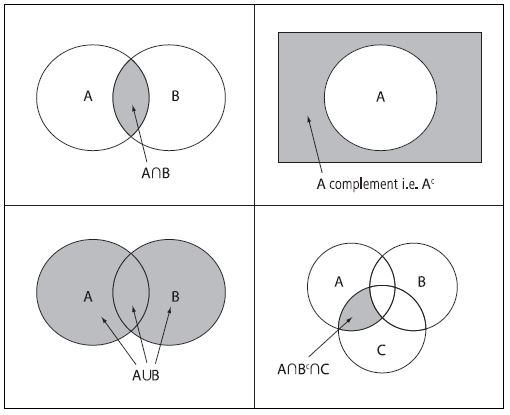
\includegraphics[width=0.7\linewidth]{venndiagram}
%
%\end{figure}

\section{Venn Diagrams}

venn diagrams
8 Disjoint Regions





%------------------------------------------------------------------------%
\end{document}
